\section{Absicherung}

\subsection{Architektur und Design}

\subsection{LISP Map Server}

\subsection{ISE / Radius}

\subsection{SGT Access List}

\subsection{Border Node}

\subsection{Fusion Router}

\subsection{DHCP}

\subsection{DNS}

\subsubsection{Infoblox HA Cluster}


\subsubsection{Read Only DNS Server an Aussenstandorten}
	
Damit Aussenstellen nicht auf DNS Server des Hauptstandortes angewiesen sind, kann in jedem Standort ein Read-Only Server betrieben werden. Somit funktioniert die Namensauflösung auch im Falle eines Kommunikationsverlusts zum Hauptstandort. 

\begin{figure}[H]
	\centering
	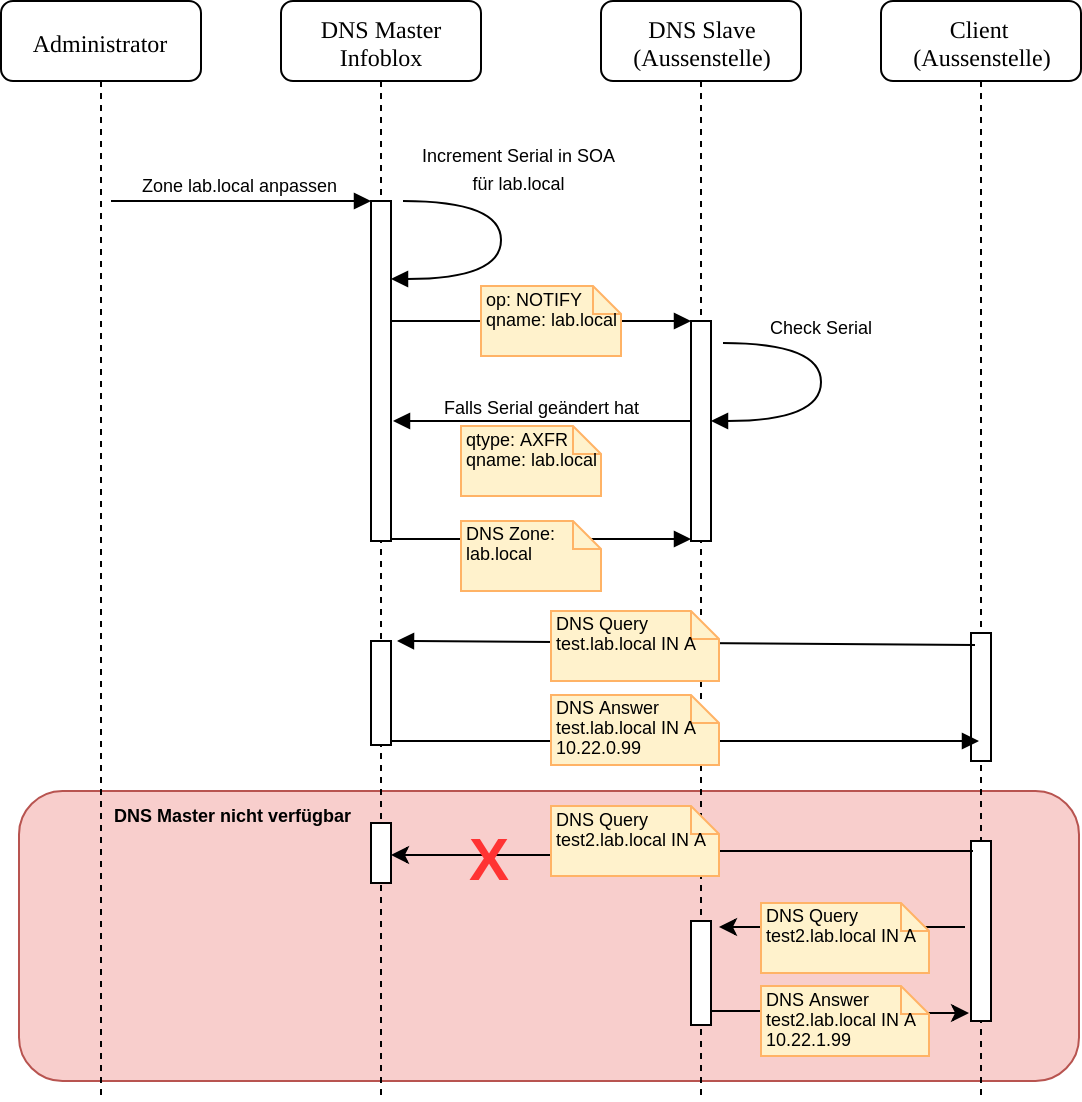
\includegraphics[width=0.8\linewidth]{img/Absicherung/DNS_Sequenzdiagram.png}
	\caption{DNS Sequenzdiagramm}
	\label{fig:DNS Sequenzdiagramm}
\end{figure}
\paragraph{Infoblox}

Damit die Read-Only Server stets über die aktuellsten DNS Zonen verfügen, müssen die Informationen von Infoblox auf diese repliziert werden. In diesem Fall wird dafür der Zone Transfer verwendet. Dazu muss dies in Infoblox für alle Slave Server erlaubt werden. 

Dies wird in Infoblox via \textit{Grid $\rightarrow$ DNS $\rightarrow$ Infoblox Instanz $\rightarrow$ Edit $\rightarrow$ Zone Transfers} ausgeführt.

\begin{figure}[H]
	\centering
	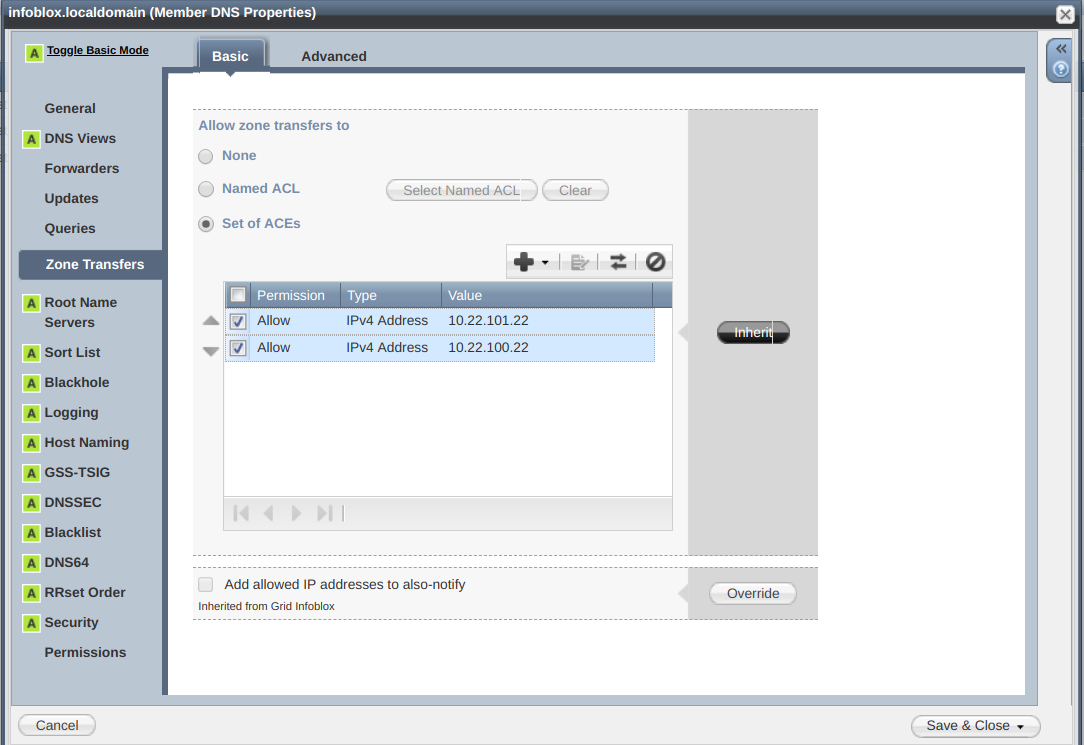
\includegraphics[width=0.8\linewidth]{img/Absicherung/Infoblox_Zone_Transfer.png}
	\caption{Infoblox Zone Transfer}
	\label{fig:Infoblox Zone Transfer}
\end{figure}

\paragraph{DNS Slaves}

Auf den Slaves an den jeweiligen Aussenstandorten müssen die Zonen als Slave Zonen konfiguriert sein und Infoblox muss als Master konfiguriert werden. Dadurch können die Zonen vom Master auf den Slave transferiert werden. Der Slave aktualisiert alle Slave Zonen in regelmässigen Abständen. Dieser Intervall wird in der Zone im SOA Record mit dem "Refresh" Parameter definiert.
Zusätzlich kann auf dem Master konfiguriert werden, dass alle Slaves mittels "Notify" informiert werden, sobald sich eine Zone ändert, worauf der Slave die aktuellsten Informationen für diese Zone abruft. Somit ist sichergestellt, dass alle Server an Aussenstandorten stets über eine aktuelle Konfiguration verfügen.

\paragraph{Clients}

Auf den Cliens ist es wichtig, dass alle nötigen DNS Server in der korrekten Reihenfolge konfiguriert werden. Als erster Server soll der Master, also Infoblox eingetragen werden. Sofern Infoblox als Cluster betrieben wird, können auch alle Instanzen des Clusters verwendet werden. Danach der Slave am jeweiligen Standort. Dies sorgt dafür, dass der Slave nur dann verwendet wird, wenn die Kommunikation zum Master nicht funktioniert.